\documentclass{report}
\usepackage{mathtools,natbib,amsmath,amsfonts}

\author{Michael Hay, Department of Earth and Space Sciences}


\begin{document}

\title{Ph.D. proposal: Mesoscale stratigraphic disturbances in ice sheets relating to plastic anisotropy}

\author{Michael Hay,
Department of Earth and Space Sciences}

\maketitle 

=======
\maketitle
\section{Introduction}
Ice cores from ice sheets provide an important record of past climate.  For accurate interpretation, a ice depth-age relationship is needed. The ice-sheet stratigraphic record is an important tool in constructing this relationship. However, ice-sheet stratigraphy can be disturbed, which can make paleoclimate interpretation difficult. Layers can be overturned, resulting in older ice lying above younger ice. As well, boudinage can occur, potentially removing layers from an ice core record. Especially on the meter or smaller scale, it is likely that a large portion of stratigraphic disruptions are due to the plastic anisotropy of ice.

Individual ice crystals have strong plastic anisotropy, deforming most easily in shear in the basal plane orthogonal to the crystallographic c-axis. Other orientations are around 100 times harder. This can lead to disturbances in several different ways. In both simple shear and vertical uniaxial compression, c-axes tend to cluster near vertical. Vertical maximum fabrics are soft under horizontal simple shear, because the basal planes are aligned with the imposed shear stress. If there is an initial open wrinkle in the stratigraphy, the enhanced simple shear can lead it to overturn into a recumbent fold \citep{throstur2002}. Boudinage can occur if there is a harder layer (under extension) surrounded by softer layers. This has likely been observed in electrical conductivity measurements at the WAIS divide core. \citet{alley97} as well found ``stripes'' of non-vertical grains in otherwise vertical-maximum fabric. Similarly, ``tilted cone`` fabrics can occur, where the maximum of the orientation distribution function is off-vertical \citep{throstur2002}. Such fabrics can lead to strain in different components than the applied deviatoric stress. This is a likely mechanism to produce smaller-scale stratigraphic disturbances, even outside of the influence of the bed. Previous work on anisotropic ice flow modeling, such as \citet{gillet2005}, has not allowed for general anisotropic viscosity. In addition, it is likely that the coupling of anisotropic flow and fabric evolution is dynamically unstable. For example, under simple shear, fabrics softer under simple shear will evolve towards a softer single maximum faster than initially harder-oriented grains. This can enhance small initial variations in fabric, and induce the formation of shear bands. In addition, \citet{montgomery-smith2011} analytically found that 3-dimensional Stokes flow of a fluid with dense rigid-fiber inclusions, whose orientation distribution function determined by Jeffery's equation, is unstable. Small nonuniformities in the orientation distribution function can grow quickly, meaning that Jeffery's equation uncoupled to flow is a poor predictor of fiber orientations. This is mathematically very similar to ice flow with fabric evolution given by Jeffery's equation (see below), except that the ice posesses nonlinear viscosity.

\section{Current work}
Studying anisotropic ice flow requires a coupled approach between fabric evolution and anisotropic flow. To this end, I have developed an strain-induced ice-fabric evolution model which incorporates a variety of physical processes. We are currently preparing a manuscript based on this model. It treats the fabric as a finite collection of grains, each with properties such as radius, dislocation density, and connectivity between different grains. Unlike previous fabric evolution models, this is mass conservative. Grains exchange mass through their nearest neighbors, and grains can grow only at the expense of others. Dynamic recrystallization is treated as probabilistic, with the probability depending on temperature and accumulated dislocation density. This is justified because there are unobserved properties which control recrystallization at subgrain scale, such as inclusions and subgrain-scale dislocation density variability. Grain rotation is given by Jeffery's equation: 

\begin{equation}
   \dot{c_i} = \zeta \left( W_{ij}  c_j + D_{ij} c_j + c_i c_j c_k D_{jk} \right)
\end{equation}

where $c_i$ is the unit vector in the direction of the c-axis, $D_{ij}$ is the strain rate tensor, and $W_{ij}$ is the spin tensor. $\zeta$ is the softness parameter, which allows for nearest neighbor interaction by effectively transferring strain.

I have forced the model with thin section data from the West Antarctice Ice Sheet (WAIS) divide ice core. Ensemble runs using bootstrapped data show that fabrics which have statistically the same distribution do not converge over time. The strengths of individual fabric realizations can oscillate with respect to other samples. This is seen in the figure using earth mover's distance as a measure of distribution distance from a perfect girdle. This occurs even if there is no recrystallization, and is likely due to the effects of grain connectivity. These differences are related to sample size. However, several hundred grains can occupy a large volume. Despite two samples being taken from the same distribution, the response to applied stress can nonetheless vary greatly. Thus, fabric variability could be an important driver behind flow disturbances. 

\section{Research plan}
By the first part of January, we will submit our manuscript regarding the fabric model. Subsequently, we will work on a coupled anisotropic flow model with a continuum fabric evolution model to look at meter-scale flow. The fabric evolution portion will use a tensor-closure approximation of the fabric in a Jeffery's-type equation \citep{jeffery1922}, in which the orientation distribution function is approximated as a series using basis functions derived from outer products of c-axis orientations. The viscosity is derived from the ODF continuum analogue of the discrete nearest neighbor interaction from \citet{throstur2002}.The flow component will be standard power-law Stokes flow, but with an anisotropic viscosity tensor represented by a $6 \times 6$ Voigt matrix generated from the fabric distribution. The strain-rate dependent factor of viscosity is assumed to be scalar. For a numerical scheme, we will likely use a simple finite-difference approach, with the fabric evolution component using an upwind method. While there is some coding difficulting inherent in it being a 3D model, the anisotropic viscosity is not difficult. I have already done much of the work in computing viscosity. The model will also use a simple cubic geometry.

This will allow us to look at numerous issues regarding anisotropic flow. Boudinage and recumbent folding from initial folds can be investigated. In addition, we will be able to test how spatial variability in ice fabric affects stratigraphy. In particular, we will see if spatial differences in fabric persist over time. We will also test whether fabric variations can produce vertical strain under horizontal simple shear. In addition, we will see if the coupled numerical model exhibits the instabilities suggested by \citet{montgomery-smith2011}. This work will shed light on conditions under which which flow disturbances can happen,and over what length scales they can disturb stratigraphy. That will allow for more accurate knowledge of the errors expected in depth-age relationships, and may allow for better dating of ice in regions of disturbed stratigraphy. The coupled finite difference model is expected to take roughly a year to develop.

As an aside to the numerical model, we may also adapt the work of \citet{montgomery-smith2011} for ice with nonlinear viscosity. It is very likely that the same instabilities occur, but the nonlinearity of viscosity may enhance the dynamic instabilities.

\begin{figure*}
\caption{90\% confidence interval and median of evolution of the distribution of the fabric sample at the top of the core, inferred from repeated bootstrap samples of the thin section data. Two sample realizations are also included.}
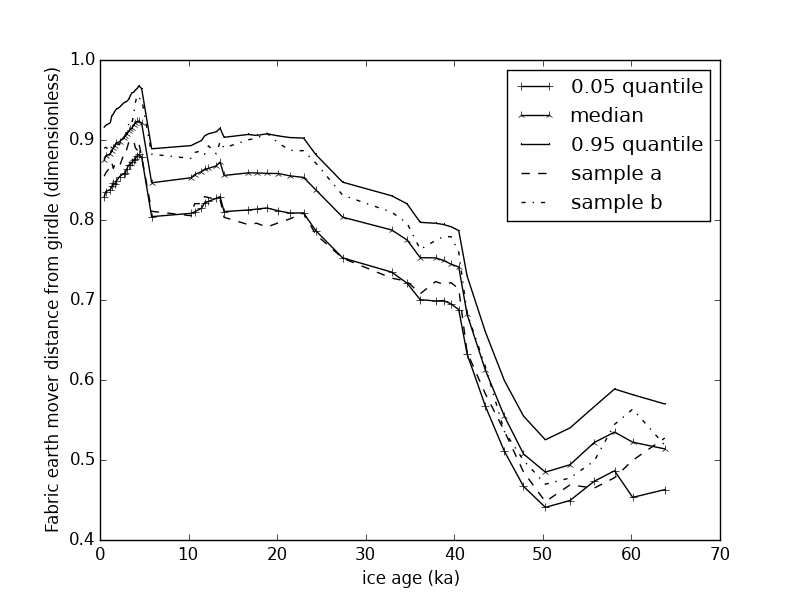
\includegraphics[width=12cm]{ci}
\end{figure*}


\subsection{Stability of anisotropic flow}

The General Orthotropic Linear Flow law (GOLF) of \citet{gillet-chaulet2005} is an analytically more tractable model for orthotropic flow. The fabric is assumed to possess three axes of symmetry, and can be described completely by its second-order orienation tensor. In a similar manner to \citet{montgomery-smith2011}, I plan to investigate the stability of orthotropic flow coupled to a fabric evolution model using linear stability analysis.

Fabric evolution is modeled using a form of the Jeffery's equation for orthotropic orientation distribution functions \citep{gillet-chaulet2006},

\begin{equation}
   \frac{\partial A_{ij}}{\partial t} = -\frac{\partial}{\partial x_k} A_{ij} u_k + W_{ik} A_{kj} - A_{ik} W_{kj} - (D_{ik}W_{kj} + D_{kj}W_{ik}) + 2 \mathbb{A}_{ijkl} C_{kl}
\end{equation}

Jeffery's equation for an orientation tensor of order $n$ depends on the orientation tensor of order $n+2$, here the fourth-order orientation tensor $\mathbb{A}_{ijkl}$. Therefore, a closure approximation for $\mathbb{A}_{ijkl}$ is required. In the literature, various approxmations are used. \citet{gillet-chaulet2006} used the "invariant-based optimal fitting closure approximation" which is is fitted based on 63 parameters. Instead, we use the quadratic closure, in which $\mathbb{A}_{ijkl} = A_{ij} A_{kl}$. This is simple, and is exact for fabrics whose c-axes are concentrated in a single orientation. 
%While this allows for a great deal of freedom to accurately fit fabrics, it would make mathematical interpretation of the results difficult. In industry, the ``hybrid closure'' is the most widely used. The hybrid closure \citep{advani90} is a weighted average between the quadratic closure ( $\mathbb{A}_{ijkl} = A_{ij} A_{kl}$ ) and the linear closure, where $\mathbb{A}_{ijkl}$ is a linear function of $A_{ij}$. This has the advantage of being mathematically simple, while being a well-attested approximation.

The consitutive relation in tensor form is given by,

\begin{equation}
S_{ij} = \eta_0 \left[ \eta_r M_{rkl} D_{kl} \left( M_{rij}^D \right)  + \eta_{r+3} \left( D_{ik} M_{rkj} + D_{kj} M_{rik} \right)^D \right],
\end{equation}

where $S_{ij}$ is the deviatoric stress tensor, and $\dot{D{ij}}$ is the strain rate tensor. $M_{rij} = v_{ri} v_{rj}$ (no sum in $r$), where $v_{ri}$ is the $r^{th}$ eigenvector of the second order orientation tensor $A_{ij}$. $\eta_r$ are six independent flow parameters, depending on $A_{ij}$ and the chosen homogenization model to transfer between the stress and strain experienced by an individual grain to that experienced by the polycrystal. Here, I assume homogeneous strain. Then, we can assume that basal glide is solely responsible for deformation, leading to the following relation between macroscopic stress and macroscopic strain rate. This leads to the inverse form of GOLF, which is a linear relationship given by,

\begin{equation}
   D_{ij} = \frac{1}{2 \eta} \left[ -2 \mathbb{A}_{ijkl}S_{kl}  S_{ik}A_{kj} + A_{ik}S{kj} \right] = H_{ijkl} S_{kl},
\end{equation}

We assume, for the unperturbed equations, that we are working in the orthotropic reference frame. Then, $A_{ij}$ become diagonal tensors of the fabric eigenvalues. Also, $M_{ij}$ reduces to $\delta_{ij}$. This simplifies EQUATION to 

\begin{equation}
   S_{ij} =\eta_0 \left[\eta_r D_{ik} \delta_{ij} +  2 \eta D_{ij} + \lambda_r D_{kk} \delta_{ij}  = L_{ijkl} D_{kl}
   \end{equation}
   
We can then substitute EQUATION into EQUATION. Due to the linearity, this can be written by composing the linear operators to get,
\begin{equation}
   D_{ij} = H_{ijkl} L_{klmn} D_{mn}
\end{equation}
The $\eta_i$ are properly fitted if the equation is satisfied for arbitary $D_{ij}$. Therefore, the composition has to yield the identity fourth order tensor. Note that $H_{ijkl}=H_{ijlk}=H_{jilk}$, and likewise for $L_{ijkl}$. Therefore, we can write this system in Voigt notation as,

\begin{equation}
   \underline{\mathbf{d}} = \underline{\underline{\mathbf{H}}} \cdot \underline{\underline{\mathbf{L}}} \cdot \underline{\mathbf{d}}
\end{equation},
where $\underline{\underline{\mathbb{H}}}$ and  $\underline{\underline{\mathbb{L}}}$  are $6 \times 6$ matrices, and $d = [D_{11},D_{22},D_{33},D_{32},D_{23},D_{21}]$. Now, in the orthotropic reference frame, it can be seen that both $H$ and $L$ are ``kite'' matrices. They have possible nonzero entries in the $3 \times 3$ submatrix in the upper left, and nonzeros on the diagonal. $\underline{\underline{\mathbb{L}}}$ is derived in \citet{golf}. They are nonunique because both $S_{ij}$ and $D_{ij}$ have zero trace.  

$\underline{\underline{\mathbf{H}}}$ is determined by the fabric eigenvalues, while $\underline{\underline{\mathbf{H}}}$ is a function of the $\eta_r$. Thus, we need to choose $\eta_r$ such that tensors with zero trace are unchanged by the transformation. $\underline{\underline{\mathbf{H}}}$ has three linearly independent components, and twelve nonzero components. It turns out that $\underline{\underline{\mathbf{H}}}^{-1}$ has 6 unique components. In the ``kite'' portion, the three nonzero components of each row are identical. The ``tail'' of the kite is trivial to invert, and it turns out that 
\begin{equation}
   \eta_{3 + i} = \frac{1}{a_j + a_k}, \text{ for } $i=1,2,3$ \text{ and } $i \neq $j,k$.
\end{equation}

Then, the remaining three $\eta_i$ can be found by,
\begin{equation}
   \eta_1 + 4 \eta_4 = -\eta_2 + 2 \eta_5 = -\eta_3 + 2 \eta_6 = const
\end{equation}
Note that we can chose the three $\lambda_i$ such that $\underline{\underline{\mathbf{H}}}^{-1} = \underline{\underline{\mathbf{L}}}$, thus this choice of $\eta_i$ exactly fits the flow law to the homogeneous stress homogenization scheme.
%  Since both To do this, note that EQUATION d is a linear relationship between $D_{ij}$ and $S_{ij}$.  
%   This expression for $S_{ij}$ can then be substituted into a linear equation $D_{ij} = C_{ijkl} S_{kl}$. The $C_{ijkl}$ tensor has six independent parameters, as a function of the non-null components of $A_{ij}$ and $\mathbb{A}_{ijkl}$ in the orthotropic frame. Written in Voigt notation, $m\mathbf{C}$ is a $6 \times 6$ kite matrix, and $m\mathbf{S}$ and $m\mathbf{D}$ are $6$-vectors. $m\mathbf{S}$ is linear function of the fabric parameters, thus  
%  Now, if we write out this equation in Voigt notation, $L_{ijkl}$ becomes a  $6 \times 6$ ``kite'' matrix. It has possible nonzero entries in the $3 \times 3$ submatrix in the upper left, and nonzeros on the diagonal.  W

To study the stability of GOLF flow in response to perturbations, I plan to do stability analysis in response to perturbations of the ODF. We assume that there is fluid obeying the GOLF flow law filling all of $\mathbb{R}^3$ with an unperturbed velocity gradient $U_{ij}$. Now, we introduce a perturbation at time $t=0$ of a specific wavenumber $\kappa$ to $A_{ij}$:

\begin{equation}
   A_{ij} \rightarrow \bar{A}_{ij} +  \epsilon \hat{A}_{ij} e^{i \kappa_k x_k}
\end{equation}

Now, in response to this initial perturbation, the quantities depending on $A_{ij}$ are perturbed by the same wavenumber:

\begin{enumerate}
   \item $u_j \rightarrow \bar{U}_{ij}x_j +  \epsilon \hat{u}_j e^{i \kappa_k x_k}$
   \item $p \rightarrow \bar{p} + \epsilon \hat{p} e^{i \kappa_k x_k}$
   \item $S_{ij} \rightarrow \bar{S}_{ij} +  \epsilon \hat{S}_{ij} e^{i \kappa_k x_k}$
   \item $\phi \rightarrow \bar{\phi} + \epsilon \hat{\phi} e^{i \kappa_k x_k}$
   \item $\mathbb{A}_{ijkl} \rightarrow \bar{\mathbb{A}}_{ijkl} + \hat{\mathbb{A}}_{ijk}$
\end{enumerate}

This is valid because we are dealing with a linear set of equations. The ``hat'' quantities are assumed to be constant over space, but may vary with time. First, to satisfy Jeffery's equation, it can be shown that at time $t$, $\kappa_j(t)=e^{-t U_{kj}} \kappa^0_k$, where $\kappa^0_k$ is the initial wavenumber at $t=0$ \citep{montgomery-smith2011}. Compressibility and force balance require

\begin{equation}
   \frac{\partial}{\partial x_j} (\hat{u}_j e^{i \kappa_k x_k}) = 0 \\ 
\end{equation}
\begin{equation}
   \frac{\partial}{\partial x_j}  (\hat{S}_{ij} - \hat{p}) e^{i \kappa_k x_k} = 0
\end{equation}

Since $\hat{S}_{ij}}$, $\hat{p}$, and $\hat{u_i}$ are spatially homogeneous, these reduce to $\kappa_k u_k = 0$ and $\kappa_k \hat{\sigma_{jk}} -\kappa_j \hat{p} = 0$, respectively. The expression for $\hat{S}_{ij}$ is found by substituting substituting in the perturbed quantities into equation  and discarding terms of $\epsilon^2$ and higher. Zero order terms vanish, as they satisfy the original equaitons. $M_{rij}$ is the product $v_{ri}v{rj}$, where , respectively, of the perturbed $A_{ij}$. The perturbed eigenvalues and eigenvectors themselves can be assumed to be linear perturbations depending on the perturbed $A_{ij}$. Therefore, the first-order perturbed Stokes equations reduce to a set of four homogeneous linear algebraic equations depending on $\hat{A}_{ij}$ and $\hat{u_k}$.

Now we look for the equation for the time evolution of the perturbation $\hat{A}_{ij}$. This is done by putting the perturbed quantities $W_{ij}$, $\D_{ij}$, $A_{ij}$, $\mathbb{A}_{ijkl}$, dividing out the exponential, and discarding higher-order terms. This yields,
\begin{equation}
\begin{align*}
   \frac{\partial \hat{A}_{ij}}{\partial t} &= -\frac{\partial}{\partial x_k} \left( \hat{A}_{ij} \bar{U_k} + \bar{A}_{ij} \hat{u}_k \right) + \bar{W}_{ik} \hat{A}_{kj} + \hat{W}_{ik} \bar{A}_{kj}  - \bar{A}_{ik} \hat{W}_{kj} 
  \\ 
   &- \hat{A}_{ik} \bar{W}_{kj} - \hat{D}_{ik}\bar{W}_{kj} - \bar{D}_{ik}\hat{W}_{kj} 
   \\ 
   & - \hat{D}_{kj}\bar{W}_{ik} - \bar{D}_{kj} \hat{W}_{ik} + 2 (\bar{\mathbb{A}}_{ijkl} \hat{D}_{kl} + \hat{\mathbb{A}}_{ijkl} \bar{D}_{kl})
\end{equation}.

Like the perturbed Stokes equations, the exponential is the only spatially nonhomogeneous component of each equation. Therefore, the perturbed Jefferys equation becomes an ordinary differential equation for six independent components of $\hat{A}_{ij}$. Alternatively, the perturbed quantities can be perturbations of the three eigenvalues, combined with a small rotation of axes of orthotropic symmetry. In that case, the perturbation of $\eta_{i+3}$ for $i=1,2,3$ is $\hat{\eta}_{i+3}= 1 - \hat{a}_j + \hat{a}_k}$, $j,k \neq i$. The other $\eta$ follow. The perturbation of the reference frame takes the form of a skew symmetric matrix whose entries are the three Euler angles of rotation. By examining the eigenvalues of the resulting system matrix, we can examine stability as a function of wavenumber, initial fabric and flow.

\subsection{Funding}
This research is currently funded by NSF Grant 0636996 for the study of anisotropic ice flow. This will continue until June 2016, although an extension is likely. If funding is needed beyond then, we will seek another grant or rely on TA funding. 

\bibliographystyle{igs}
\bibliography{anis}

\end{document}
